% Drawing 74/05-19 -- folder 74, batch 05, archive page 100 (PDF page 101).
% Transcription: Une étoile de triangles : plusieurs triangles ayant un sommet commun, disposés en roue.
% Kind: star of triangles (inline). Method 2 (schematic redraw from the facsimile). Status: ok.
% Notes: Inside the line of text « (... ) »: several thin triangles with a common vertex arranged as a wheel; drawn as four wedges and two spokes.
% Coordinates: 1 unit = 1 mm = 1/100 of the crop width (bbox in page fractions: [0.3, 0.75, 0.7, 0.9]).
% Redrawn by Claude (claude-opus-5-5), issue #73, 2026-11-07; not checked by a human; not compiled (no TeX in the session).
% Rights: reproduces part of the work -- behind RENDER_TRANSCRIPTS, never published by itself.
\documentclass[tikz,border=3pt]{standalone}
\usepackage{amsmath,amssymb}
\usetikzlibrary{patterns,arrows.meta}
\tikzset{pencil/.style={black!45}, struck/.style={black!35}, mark/.style={circle,draw,inner sep=1.3pt}, pt/.style={circle,fill,inner sep=0.9pt}, opt/.style={circle,draw,fill=white,inner sep=1.1pt}}
\begin{document}
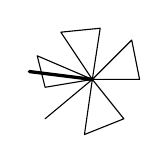
\begin{tikzpicture}[x=1mm,y=1mm,line cap=round,line join=round,font=\scriptsize]
\draw (53,-30) -- (46,-27) -- (47,-31) -- cycle;
\draw (53,-30) -- (49,-24) -- (54,-23.5) -- cycle;
\draw (53,-30) -- (58,-25) -- (59,-30) -- cycle;
\draw (53,-30) -- (57,-35) -- (52,-37) -- cycle;
\draw (53,-30) -- (47,-35);
\draw[very thick] (53,-30) -- (45,-29);
\end{tikzpicture}
\end{document}
